\subsection{Spatio-Temporal Detection}
\begin{frame}[allowframebreaks]{Spatio-Temporal Detection}
    \textbf{Problem Statement:} \\
    Given a long untrimmed video, the goal is to detect all people in both space and time, and classify the activities they are performing.

    \begin{itemize}
        \item \textbf{Input:} Untrimmed video sequence.
        \item \textbf{Output:} For each person, a spatio-temporal tube (bounding boxes across frames) and an activity label.
    \end{itemize}
\framebreak
    \textbf{Example: AVA Dataset} \\
    The AVA (Atomic Visual Actions) dataset provides annotated videos with bounding boxes and action labels for each person in every frame.

    \begin{figure}
        \centering
        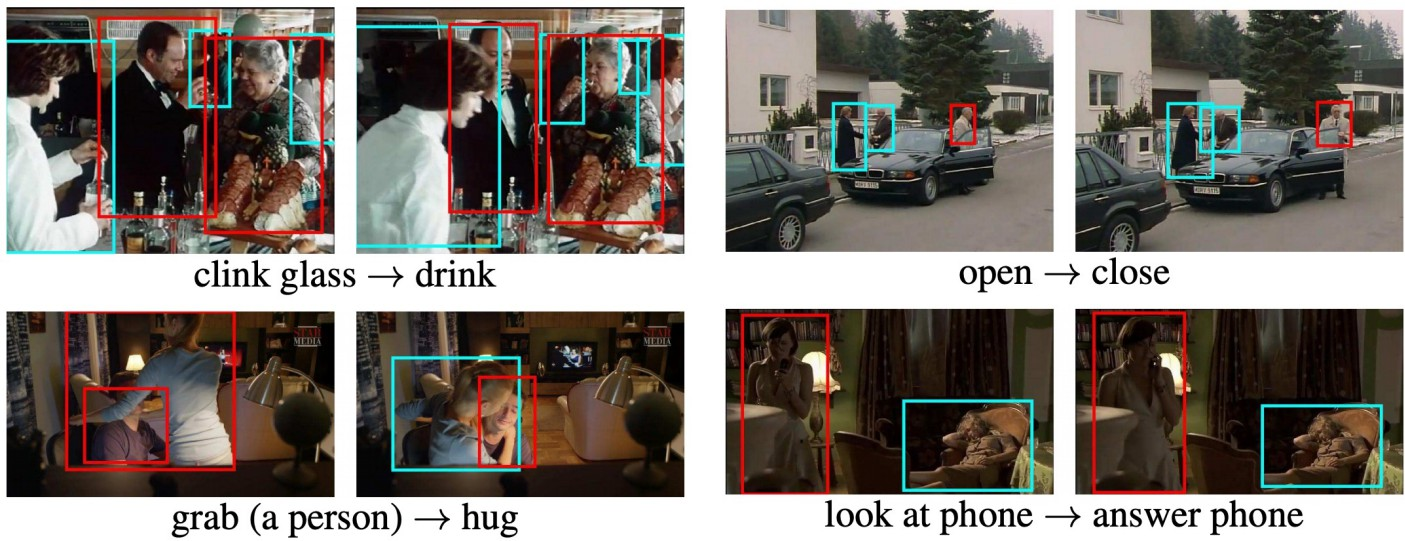
\includegraphics[width=1\textwidth,height=0.9\textheight,keepaspectratio]{images/video/slide_40_1_img.jpg}
    \end{figure}
    \begin{itemize}
        \item \textbf{Annotations:} Spatial (bounding boxes) and temporal (frame-level) localization of actions.
    \end{itemize}
\framebreak
    \textbf{Spatio-temporal detection} involves identifying and localizing objects or events in both space and time within video sequences. This is crucial for tasks such as action recognition, event detection, and video surveillance.

    \begin{itemize}
        \item \textbf{Spatio-Temporal Features:} These features capture both the spatial layout of objects and their temporal dynamics.
        \item \textbf{3D Convolutional Networks (3D CNNs):} Extend traditional CNNs by adding a temporal dimension, allowing them to learn spatio-temporal patterns directly from video data.
        \item \textbf{Challenges:} High computational cost, data sparsity, and the need for large annotated datasets.
        \item \textbf{Applications:} Surveillance, human-computer interaction, sports analytics.
    \end{itemize}
\end{frame}